% cpu/overheads.tex
% SPDX-License-Identifier: CC-BY-SA-3.0

\section{Overheads}
\label{sec:cpu:Overheads}

이 섹션에서는 앞의 섹션에서 나열했던 장애들의 실제 성능에의 오버헤드를
보입니다.
하지만, 그 전에 하드웨어 시스템 아키텍쳐에 대해서 간략히 알아볼 필요가 있는데,
다음 섹션에서 이를 다룹니다.
\iffalse

This section presents actual overheads of the obstacles to performance
listed out in the previous section.
However, it is first necessary to get a rough view of hardware system
architecture, which is the subject of the next section.
\fi

\subsection{Hardware System Architecture}
\label{sec:cpu:Hardware System Architecture}

\begin{figure}[tb]
\centering
\resizebox{3in}{!}{\includegraphics{cpu/SystemArch}}
\caption{System Hardware Architecture}
\label{fig:cpu:System Hardware Architecture}
\end{figure}

Figure~\ref{fig:cpu:System Hardware Architecture} 는 8 코어 컴퓨터 시스템의
간략한 구조를 보여줍니다.
각 다이는 CPU 코더 한쌍을 가지고 있고, 각 코어는 캐시를 갖고, 각 캐시는 쌍을
이루는 코어와 통신을 할 수 있도록 하는 연결이 되어 있습니다.
그림 중간의 system interconnect 는 네개의 다이가 통신할 수 있도록 하고, 메인
메모리로 각 다이를 연결합니다.

이 시스템에서 데이터는 하나의 2의 승수로 정렬된 메모리의 블락들로, 보통 32 에서
256 바이트 사이인 ``캐시 라인'' 단위로 움직입니다.
한 CPU 는 메모리로부터 자신의 레지스터로 변수를 가져오려면, 그 변수를 가지고
있는 캐시 라인을 자신의 캐시로 가져와야 합니다.
비슷하게, 한 CPU 는 자신의 레지스터로부터 메모리로 어떤 값을 쓰려 할 때, 일단
그 변수를 담고 있는 캐시 라인을 자신의 캐시로 가져와야 합니다만, 또한 다른 CPU
가 그 캐시 라인의 카피를 들고 있지 않음을 보장해야 합니다.

예를 들어, 만약 CPU~0 CPU~7 의 캐시에 있는 캐시라인에 있는 변수에
compare-and-swap (CAS) 오퍼레이션을 하려 하면, 다음의 간략화한 이벤트들이
일어날 겁니다:

\iffalse
Figure~\ref{fig:cpu:System Hardware Architecture}
shows a rough schematic of an eight-core computer system.
Each die has a pair of CPU cores, each with its cache, as well as an
interconnect allowing the pair of CPUs to communicate with each other.
The system interconnect in the middle of the diagram allows the
four dies to communicate, and also connects them to main memory.

Data moves through this system in units of ``cache lines'', which
are power-of-two fixed-size aligned blocks of memory, usually ranging
from 32 to 256 bytes in size.
When a CPU loads a variable from memory to one of its registers, it must
first load the cacheline containing that variable into its cache.
Similarly, when a CPU stores a value from one of its registers into
memory, it must also load the cacheline containing that variable into
its cache, but must also ensure that no other CPU has a copy of that
cacheline.

For example, if CPU~0 were to perform a compare-and-swap (CAS) operation on a
variable whose cacheline resided in CPU~7's cache, the following
over-simplified sequence of events might ensue:
\fi

\begin{enumerate}
\item	CPU~0 는 자신의 로컬 캐시를 확인하고, 그 캐시라인이 없음을 발견합니다.
\item	요청은 CPU~0 와 CPU~1 사이의 연결로 넘겨져서 CPU~1 의 로컬 캐시를
	확인해봅니다만, 역시 해당 캐시라인이 없음을 발견합니다.
\item	요청은 시스템 연결부로 넘겨지고, 다른 세개의 다이들을 체크합니다. 결과,
	해당 캐시라인은 CPU~6과 CPU~7 이 위치한 다이에 있음을 확인합니다.
\item	요청은 CPU~6 과 CPU~7 연결부로 넘겨져 각 CPU 의 캐시를 확인해 해당 캐시
	라인이 CPU~7 의 캐시에 있음을 발견합니다.
\item	CPU~7 은 해당 캐시라인을 자신의 연결부로 넘기고, 자신의 캐시에서 해당
	캐시라인을 비워버립니다.
\item	CPU~6 와 CPU~7 의 연결부는 해당 캐시 라인을 시스템 연결부로 넘깁니다.
\item	시스템 연결부는 해당 캐시 라인을 CPU~0 과 CPU~1 연결부로 넘깁니다.
\item	CPU~0 과 CPU~1 연결부는 해당 캐시라인을 CPU~0 의 캐시로 보냅니다.
\item	CPU~0 는 이제 자신의 캐시 안에 있는 변수에 CAS 오퍼레이션을 수행할 수
	있습니다.
\end{enumerate}

\iffalse
\begin{enumerate}
\item	CPU~0 checks its local cache, and does not find the cacheline.
\item	The request is forwarded to CPU~0's and 1's interconnect,
	which checks CPU~1's local cache, and does not find the cacheline.
\item	The request is forwarded to the system interconnect, which
	checks with the other three dies, learning that the cacheline
	is held by the die containing CPU~6 and 7.
\item	The request is forwarded to CPU~6's and 7's interconnect, which
	checks both CPUs' caches, finding the value in CPU~7's cache.
\item	CPU~7 forwards the cacheline to its interconnect, and also
	flushes the cacheline from its cache.
\item	CPU~6's and 7's interconnect forwards the cacheline to the
	system interconnect.
\item	The system interconnect forwards the cacheline to CPU~0's and 1's
	interconnect.
\item	CPU~0's and 1's interconnect forwards the cacheline to CPU~0's
	cache.
\item	CPU~0 can now perform the CAS operation on the value in its cache.
\end{enumerate}
\fi

\QuickQuiz{}
	이제 \emph{간략화된} 거라구요?
	이것보다 더 복잡한게 어떻게 \emph{가능하죠}?
	\iffalse
	This is a \emph{simplified} sequence of events?
	How could it \emph{possibly} be any more complex?
	\fi
\QuickQuizAnswer{
	이 예는 다음을 포함해 몇가지 가능한 복잡한 경우를 뺐습니다:
	\begin{enumerate}
	\item	해당 캐시라인에 대해 다른 CPU 들도 동사에 CAS 오퍼레이션을
		수행하려 하고 있을 수 있습니다.
	\item	해당 캐시라인은 리드 온리로 다른 CPU 들의 캐시들에 복사되어
		있을 수 있는데, 이 경우엔 그 캐시들도 비워야 할 필요가
		생깁니다.
	\item	CPU~7 은 해당 요청이 도착했을 때 해당 캐시 라인에 뭔가 연산을
		수행하고 있었을 수 있고, 이 경우 CPU~7 은 자신의 연산이 끝날
		때까지 해당 요청을 잠시 대기하고 있게 해야 합니다.
	\item	CPU~7 은 (예를 들어, 다른 데이터를 위한 공간을 만들기 위해)
		해당 캐시라인을 캐시에서 없앴을 수 있고, 이로 인해 요청이
		도착한 시점에서는 캐시라인이 메모리에 있을 수 있습니다.
	\item	캐시라인에서 고칠 수 있는 에러가 났을 수 있는데, 그렇다면 해당
		데이터가 사용되기 전에 그 에러는 고쳐져야 합니다.
	\iffalse
	This sequence ignored a number of possible complications,
	including:

	\begin{enumerate}
	\item	Other CPUs might be concurrently attempting to perform
		CAS operations involving this same cacheline.
	\item	The cacheline might have been replicated read-only in
		several CPUs' caches, in which case, it would need to
		be flushed from their caches.
	\item	CPU~7 might have been operating on the cache line when
		the request for it arrived, in which case CPU~7 might
		need to hold off the request until its own operation
		completed.
	\item	CPU~7 might have ejected the cacheline from its cache
		(for example, in order to make room for other data),
		so that by the time that the request arrived, the
		cacheline was on its way to memory.
	\item	A correctable error might have occurred in the cacheline,
		which would then need to be corrected at some point before
		the data was used.
	\fi
	\end{enumerate}

	제품 품질의 캐시 일관성 메커니즘들은 이런 종류의 여러 복잡한
	경우~\cite{Hennessy95a,DavidECuller1999,MiloMKMartin2012scale,DanielJSorin2011MemModel}
	때문에 엄청나게 복잡합니다.

	\iffalse
	Production-quality cache-coherence mechanisms are extremely
	complicated due to these sorts of
	considerations~\cite{Hennessy95a,DavidECuller1999,MiloMKMartin2012scale,DanielJSorin2011MemModel}.
	\fi
%
} \QuickQuizEnd

\QuickQuiz{}
	왜 CPU~7 의 캐시에서 해당 캐시라인을 비워야 하죠?

	\iffalse
	Why is it necessary to flush the cacheline from CPU~7's cache?
	\fi
\QuickQuizAnswer{
	만약 해당 캐시라인이 CPU~7 의 캐시에서 비워지지 않는다면, CPU~0 과
	CPU~7 은 같은 변수에 대해 서로 다른 값을 보게 될 겁니다.
	이런 종류의 비일관성은 병렬 소프트웨어를 매우 복잡하게 만들 수 있고,
	때문에 하드웨어 설계자들은 그런 문제를 없애려 노력해 왔습니다.
	\iffalse
	If the cacheline was not flushed from CPU~7's cache, then
	CPUs~0 and 7 might have different values for the same set
	of variables in the cacheline.
	This sort of incoherence would greatly complicate parallel
	software, and so hardware architects have been convinced to
	avoid it.
	\fi
} \QuickQuizEnd

이 간략화된 시나리오는
Appendix~\ref{chp:app:whymb:Why Memory Barriers?} 에서 자세히 설명되는
\emph{캐시 코히런시
프로토콜}~\cite{Hennessy95a,DavidECuller1999,MiloMKMartin2012scale,DanielJSorin2011MemModel}
의 시작일 뿐입니다.
CAS 오퍼레이션으로 시작되는 이벤트 시퀀스에서 볼 수 있듯이, 하나의 인스트럭션이
상당한 양의 프로토콜 트래픽을 일으킬 수 있으며, 이는 병렬 프로그램의 성능을
상당히 떨어뜨릴 수 있습니다.

다행히도, 특정 변수가 업데이트 되지 않는 시간 간격동안 자주 읽혀지게 된다면,
해당 변수는 모든 CPU 들의 캐시 위에 복사될 수 있습니다.
이 복사는 모든 CPU 들이 이 \emph{읽기가 대부분인} 변수로의 매우 빠른 접근을
즐길 수 있도록 해줄 겁니다.
Chapter~\ref{chp:Deferred Processing} 는 이 중요한 하드웨어의 읽기가 대부분인
경우의 최적화의 장점을 최대한 취하는 동기화 메커니즘들을 소개합니다.
\iffalse

This simplified sequence is just the beginning of a discipline called
\emph{cache-coherency protocols}~\cite{Hennessy95a,DavidECuller1999,MiloMKMartin2012scale,DanielJSorin2011MemModel},
which is discussed in more detail in
Appendix~\ref{chp:app:whymb:Why Memory Barriers?}.
As can be seen in the sequence of events triggered by a CAS operation,
a single instruction can cause considerable protocol traffic, which
can significantly degrade your parallel program's performance.

Fortunately, if a given variable is being frequently read during a time
interval during which it is never updated, that variable can be replicated
across all CPUs' caches.
This replication permits all CPUs to enjoy extremely fast access to
this \emph{read-mostly} variable.
Chapter~\ref{chp:Deferred Processing} presents synchronization
mechanisms that take full advantage of this important hardware read-mostly
optimization.
\fi

\subsection{Costs of Operations}
\label{sec:cpu:Costs of Operations}

\begin{table}
\rowcolors{1}{}{lightgray}
\renewcommand*{\arraystretch}{1.1}
\centering\small
\begin{tabular}
  {
    l
    S[table-format = 9.1]
    S[table-format = 9.1]
  }
	\toprule
	Operation		& \multicolumn{1}{r}{Cost (ns)}
			& {\parbox[b]{.7in}{\raggedleft Ratio\\(cost/clock)}} \\
	\midrule
	Clock period		&           0.6	&           1.0 \\
	Best-case CAS		&          37.9	&          63.2 \\
	Best-case lock		&          65.6	&         109.3 \\
	Single cache miss	&         139.5	&         232.5 \\
	CAS cache miss		&         306.0	&         510.0 \\
	Comms Fabric		&       5 000	&       8 330	\\
	Global Comms		& 195 000 000	& 325 000 000   \\
	\bottomrule
\end{tabular}
\caption{Performance of Synchronization Mechanisms on 4-CPU 1.8\,GHz AMD Opteron 844 System}
\label{tab:cpu:Performance of Synchronization Mechanisms on 4-CPU 1.8GHz AMD Opteron 844 System}
\end{table}

병렬 프로그램에 중요하고 흔히 사용되는 오퍼레이션의 오버헤드들이
Table~\ref{tab:cpu:Performance of Synchronization Mechanisms on 4-CPU 1.8GHz
AMD Opteron 844 System} 에 표시되어 있습니다.
이 시스템의 클락 시간은 약 0.6ns 입니다.
많은 근래의 마이크로프로세서가 한 클락 시간동안 여러 인스트럭션을 수행 완료시킬
수 있긴 합니다만, 모든 오퍼레이션의 비용은 클락 시간을 기준으로 해서 ``Ratio''
라고 표시한 세번째 행의 값으로 나타낼 수 있습니다.
이 표에 대해서 가장 먼저 알아둬야 할 것은, 큰 비율의 값들입니다.

\iffalse
The overheads of some common operations important to parallel programs are
displayed in
Table~\ref{tab:cpu:Performance of Synchronization Mechanisms on 4-CPU 1.8GHz AMD Opteron 844 System}.
This system's clock period rounds to 0.6\,ns.
Although it is not unusual for modern microprocessors to be able to
retire multiple instructions per clock period, the operations's costs are
nevertheless normalized to a clock period in the third column, labeled
``Ratio''.
The first thing to note about this table is the large values of many of
the ratios.
\fi

최선의 경우 compare-and-swap (CAS) 오퍼레이션은 클락 시간보다 60배 이상 큰, 약
40 나노세컨드를 소비합니다.
여기서 ``최선의 경우'' 는 한 변수에 CAS 오퍼레이션을 수행하는 CPU와 해당 변수를
마지막으로 건든 CPU가 동일해서 관련된 캐시 라인이 이미 자신의 캐시 안에 있는
경우입니다.
비슷하게, 최선의 경우 락 오퍼레이션 (락 획득과 해제 두개 오퍼레이션의 수행
시간의 합) 은 60 나노 세컨드가 넘고 100 클락 사이클이 넘는  시간을 소비합니다.
다시 말하지만, ``최선의 경우'' 는 락을 나타내는 데이터 구조가 이미 락의 획득과
해제를 수행하는 CPU 의 캐시 위에 있는 경우입니다.
락 오퍼레이션은 락 데이터 구조에 대한 두번의 어토믹 오퍼레이션을 필요로 하기
때문에 CAS 보다 비쌉니다.

\iffalse
The best-case compare-and-swap (CAS) operation consumes almost forty
nanoseconds, a duration more than sixty times that of the clock period.
Here, ``best case'' means that the same CPU now performing the CAS operation
on a given variable was the last CPU to operate on this variable, so
that the corresponding cache line is already held in that CPU's cache.
Similarly, the best-case lock operation (a ``round trip'' pair consisting
of a lock acquisition followed by a lock release) consumes more than
sixty nanoseconds, or more than one hundred clock cycles.
Again, ``best case'' means that the data structure representing the
lock is already in the cache belonging to the CPU acquiring and releasing
the lock.
The lock operation is more expensive than CAS because it requires two
atomic operations on the lock data structure.
\fi

캐시 미스가 난 오퍼레이션은 거의 200 클락 사이클인 140 나노세컨드를 소모합니다.
이 캐시 미스 비용 측정을 위해 사용된 코드는 미스가 난 데이터를 다른 CPU 의
캐시에서 얻어옵니다. 즉, 이 캐시 미스 오퍼레이션은 메모리까지 접근하지는
않습니다.
변수의 기존 값을 보는 것은 물론, 새로운 값을 쓰기도 해야 하는 CAS 오퍼레이션은
500 클락 사이클인 300 나노세컨드를 소비합니다.
이걸 조금 생각해 봅시다.
CPU 는 \emph{하나의} CAS 오퍼레이션을 수행하는데 필요한 시간 동안, \emph{500
개의} 보통 인스트럭션을 수행할 수도 있었습니다.
이건 fine-grained 락킹만이 아니라 fine-grained 전역적 규칙에 기반한 모든 동기화
메커니즘의 한계를 보여줍니다.

\iffalse
An operation that misses the cache consumes almost one hundred and forty
nanoseconds, or more than two hundred clock cycles.
The code used for this cache-miss measurement passes the cache line
back and forth between a pair of CPUs, so this cache miss is satisfied
not from memory, but rather from the other CPU's cache.
A CAS operation, which must look at the old value of the variable as
well as store a new value, consumes over three hundred nanoseconds, or
more than five hundred clock cycles.
Think about this a bit.
In the time required to do \emph{one} CAS operation, the CPU could have
executed more than \emph{five hundred} normal instructions.
This should demonstrate the limitations not only of fine-grained locking,
but of any other synchronization mechanism relying on fine-grained
global agreement.
\fi

\QuickQuiz{}
	하드웨어 설계자들은 분명 이 상황을 개선하려 노력할 수 있었을 거예요!
	왜 그들은 이 단일 인스트럭션 오퍼레이션들의 끔찍한 성능을 만족하고
	있는거죠?
	\iffalse
	Surely the hardware designers could be persuaded to improve
	this situation!
	Why have they been content with such abysmal performance
	for these single-instruction operations?
	\fi
\QuickQuizAnswer{
	하드웨어 설계자들은 이 문제를 해결하려 노력\emph{했었}습니다만,
	물리학자 스티븐 호킹 정도의 권위자에게만 조언을 얻었습니다.
	호킹은 하드웨어 설계자들이 두개의 기본 문제~\cite{BryanGardiner2007}를
	가지고 있음을 발견했습니다:

	\begin{enumerate}
	\item	빛의 한계 속도, 그리고
	\item	물질의 원자적 본성.
	\end{enumerate}

	\iffalse
	The hardware designers \emph{have} been working on this
	problem, and have consulted with no less a luminary than
	the physicist Stephen Hawking.
	Hawking's observation was that the hardware designers have
	two basic problems~\cite{BryanGardiner2007}:

	\begin{enumerate}
	\item	the finite speed of light, and
	\item	the atomic nature of matter.
	\end{enumerate}
	\fi

\begin{table}
\rowcolors{1}{}{lightgray}
\renewcommand*{\arraystretch}{1.1}
\centering\small
\begin{tabular}
  {
    l
    S[table-format = 9.1]
    S[table-format = 9.1]
  }
	\toprule
	Operation		& \multicolumn{1}{r}{Cost (ns)}
			& {\parbox[b]{.7in}{\raggedleft Ratio\\(cost/clock)}} \\
	\midrule
	Clock period		&           0.4	&           1.0 \\
	``Best-case'' CAS	&          12.2	&          33.8 \\
	Best-case lock		&          25.6	&          71.2 \\
	Single cache miss	&          12.9	&          35.8 \\
	CAS cache miss		&           7.0	&          19.4 \\
	\midrule
	Off-Core		&		&		\\
	Single cache miss	&          31.2	&          86.6 \\
	CAS cache miss		&          31.2	&          86.5 \\
	\midrule
	Off-Socket		&		&		\\
	Single cache miss	&          92.4	&         256.7 \\
	CAS cache miss		&          95.9	&         266.4 \\
	Comms Fabric		&       2 600   &       7 220   \\
	Global Comms		& 195 000 000	& 542 000 000   \\
	\bottomrule
\end{tabular}
\caption{Performance of Synchronization Mechanisms on 16-CPU 2.8\,GHz Intel X5550 (Nehalem) System}
\label{tab:cpu:Performance of Synchronization Mechanisms on 16-CPU 2.8GHz Intel X5550 (Nehalem) System}
\end{table}

	첫번째 문제는 기본 속도를 제한하고, 두번째 문제는 동작의 소형화를
	제한하여 결과적으로 단위시간당 가능한 오퍼레이션의 갯수를 제한합니다.
	그리고 이 문제는 설령, 현재 상품화된 CPU 들의 속도를 10 GHz 아래로
	제한하고 있는, 에너지 소비 문제를 피해간다 해도 존재합니다.

	Table~\ref{tab:cpu:Performance of Synchronization Mechanisms on 16-CPU
	2.8GHz Intel X5550 (Nehalem) System} 과
	페이지~\pageref{tab:cpu:Performance of Synchronization Mechanisms on
	4-CPU 1.8GHz AMD Opteron 844 System} 의 Table~\ref{tab:cpu:Performance
	of Synchronization Mechanisms on 4-CPU 1.8GHz AMD Opteron 844 System}
	를 비교해 보면 알 수 있겠지만, 분명 개선은 이루어지고 있습니다.
	하드웨어 쓰레드들을 단일 코어에 집어넣고 복수의 코어들을 하나의 다이에
	넣는 것은 적어도 싱글 코어내에서 또는 단일 다이 내에서의 반응속도는
	엄청나게 개선했습니다.
	전체 시스템 반응속도에서도 일부 개선이 있었습니다만, 겨우 대략 두배
	정도입니다.
	안타깝지만, 지난 몇년간 빛의 속도나 물질의 원자성의 본질은 변하지
	않았습니다.

	Section~\ref{sec:cpu:Hardware Free Lunch?} 에서는 병렬 프로그래머들의
	곤경을 완화시키기 위해 어떤 일을 해줄 수 있을지 알아봅니다.

	\iffalse
	The first problem limits raw speed, and the second limits
	miniaturization, which in turn limits frequency.
	And even this sidesteps the power-consumption issue that
	is currently holding production frequencies to well below
	10\,GHz.

	Nevertheless, some progress is being made, as may be seen
	by comparing
	Table~\ref{tab:cpu:Performance of Synchronization Mechanisms on 16-CPU 2.8GHz Intel X5550 (Nehalem) System}
	with
	Table~\ref{tab:cpu:Performance of Synchronization Mechanisms on 4-CPU 1.8GHz AMD Opteron 844 System}
	on
	page~\pageref{tab:cpu:Performance of Synchronization Mechanisms on 4-CPU 1.8GHz AMD Opteron 844 System}.
	Integration of hardware threads in a single core and multiple
	cores on a die have improved latencies greatly, at least within the
	confines of a single core or single die.
	There has been some improvement in overall system latency,
	but only by about a factor of two.
	Unfortunately, neither the speed of light nor the atomic nature
	of matter has changed much in the past few years.

	Section~\ref{sec:cpu:Hardware Free Lunch?}
	looks at what else hardware designers might be
	able to do to ease the plight of parallel programmers.
	\fi
} \QuickQuizEnd

I/O 오퍼레이션들은 이보다도 더 비쌉니다.
``Comms Fabric'' 열에서 나타나 있듯이, InfiniBand 나 몇몇 독점 연결장치와 같은
고성능의 (그리고 고비용의!) 통신 장치들은 5 \emph{천개}의 인스트럭션이 수행될
수도 있는, 약 3 마이크로세컨드의 대기시간을 갖습니다.
표준에 기반한 통신 네트워크들은 종종 몇몇 프로토콜 프로세싱을 필요로 하고, 이는
대기시간을 더욱 증가시킵니다. 물론, 지형적 거리도 대기시간을 늘립니다.
이론적으로 빛의 속도라고 해도 지구를 한바퀴 돌기 위해선 약 130
\emph{밀리세컨드} 의 시간을 필요로 합니다. 이는 2억 클락 사이클 이상입니다. 이
수치는 ``Global Comms'' 열에 있습니다.

\iffalse
I/O operations are even more expensive.
As shown in the ``Comms Fabric'' row,
high performance (and expensive!) communications fabric, such as
InfiniBand or any number of proprietary interconnects, has a latency
of roughly five microseconds for an end-to-end round trip, during which
time more than eight \emph{thousand} instructions might have been executed.
Standards-based communications networks often require some sort of
protocol processing, which further increases the latency.
Of course, geographic distance also increases latency, with the
speed-of-light through optical fiber latency around the world coming to
roughly 195 \emph{milliseconds}, or more than 300 million clock
cycles, as shown in the ``Global Comms'' row.
\fi

% Reference of Infiniband latency:
% http://www.hpcadvisorycouncil.com/events/2014/swiss-workshop/presos/Day_1/1_Mellanox.pdf
%     page 6/76 'Leading Interconnect, Leading Performance'

\QuickQuiz{}
	숫자가 미친듯이 크군요!
	어떡해야 제 머리로 이걸 이해할 수 있을까요?
	\iffalse
	These numbers are insanely large!
	How can I possibly get my head around them?
	\fi
\QuickQuizAnswer{
	휴지 한 롤을 가져오세요.
	미제 휴지라면, 한 롤의 휴지는 약 350-500 조각의 휴지로 구성됩니다.
	한개 조각이 하나의 클락 사이클이라고 생각하고, 휴지를 모두 풀어 보세요.

	그게 하나의 CAS 캐시 미스를 의미한다고 보면 됩니다.

	더 비싼 시스템간 커뮤니케이션 대기시간을 보려면, 몇개의 휴지 롤 (또는
	여러 휴지 케이스들) 이 필요할 겁니다.

	중요한 팁 하나: 당신이 살아가면서 필요한 휴지가 얼마나 되는지도
	생각해보세요!

	\iffalse
	Get a roll of toilet paper.
	In the USA, each roll will normally have somewhere around
	350-500 sheets.
	Tear off one sheet to represent a single clock cycle, setting it aside.
	Now unroll the rest of the roll.

	The resulting pile of toilet paper will likely represent a single
	CAS cache miss.

	For the more-expensive inter-system communications latencies,
	use several rolls (or multiple cases) of toilet paper to represent
	the communications latency.

	Important safety tip: make sure to account for the needs of
	those you live with when appropriating toilet paper!
	\fi
} \QuickQuizEnd

\subsection{Hardware Optimizations}
\label{sec:cpu:Hardware Optimizations}

It is only natural to ask how the hardware is helping, and the answer
is ``Quite a bit!''

One hardware optimization is large cachelines.
This can provide a big performance boost, especially when software is
accessing memory sequentially.
For example, given a 64-byte cacheline and software accessing 64-bit
variables, the first access will still be slow due to speed-of-light
delays (if nothing else), but the remaining seven can be quite fast.
However, this optimization has a dark side, namely false sharing,
which happens when different variables in the same cacheline are
being updated by different CPUs, resulting in a high cache-miss rate.
Software can use the alignment directives available in many compilers
to avoid false sharing, and adding such directives is a common step
in tuning parallel software.

A second related hardware optimization is cache prefetching, in which
the hardware reacts to consecutive accesses by prefetching subsequent
cachelines, thereby evading speed-of-light delays for these
subsequent cachelines.
Of course, the hardware must use simple heuristics to determine when
to prefetch, and these heuristics can be fooled by the complex data-access
patterns in many applications.
Fortunately, some CPU families allow for this by providing special
prefetch instructions.
Unfortunately, the effectiveness of these instructions in the general
case is subject to some dispute.

A third hardware optimization is the store buffer, which allows a string
of store instructions to execute quickly even when the stores are to
non-consecutive addresses and when none of the needed cachelines are
present in the CPU's cache.
The dark side of this optimization is memory misordering, for which see
Chapter~\ref{chp:Advanced Synchronization: Memory Ordering}.

A fourth hardware optimization is speculative execution, which can
allow the hardware to make good use of the store buffers without
resulting in memory misordering.
The dark side of this optimization can be energy inefficiency and
lowered performance if the speculative execution goes awry and must
be rolled back and retried.

A fifth hardware optimization is large caches, allowing individual
CPUs to operate on larger datasets without incuring expensive cache
misses.
Although large caches can degrade energy efficiency and cache-miss
latency, the ever-growing cache sizes on production microprocessors
attests to the power of this optimization.

A final hardware optimization is read-mostly replication, in which
data that is frequently read but rarely updated is present in all
CPUs' caches.
This optimization allows the read-mostly data to be accessed
exceedingly efficiently, and is the subject of
Chapter~\ref{chp:Deferred Processing}.

\begin{figure}[tb]
\centering
\resizebox{3in}{!}{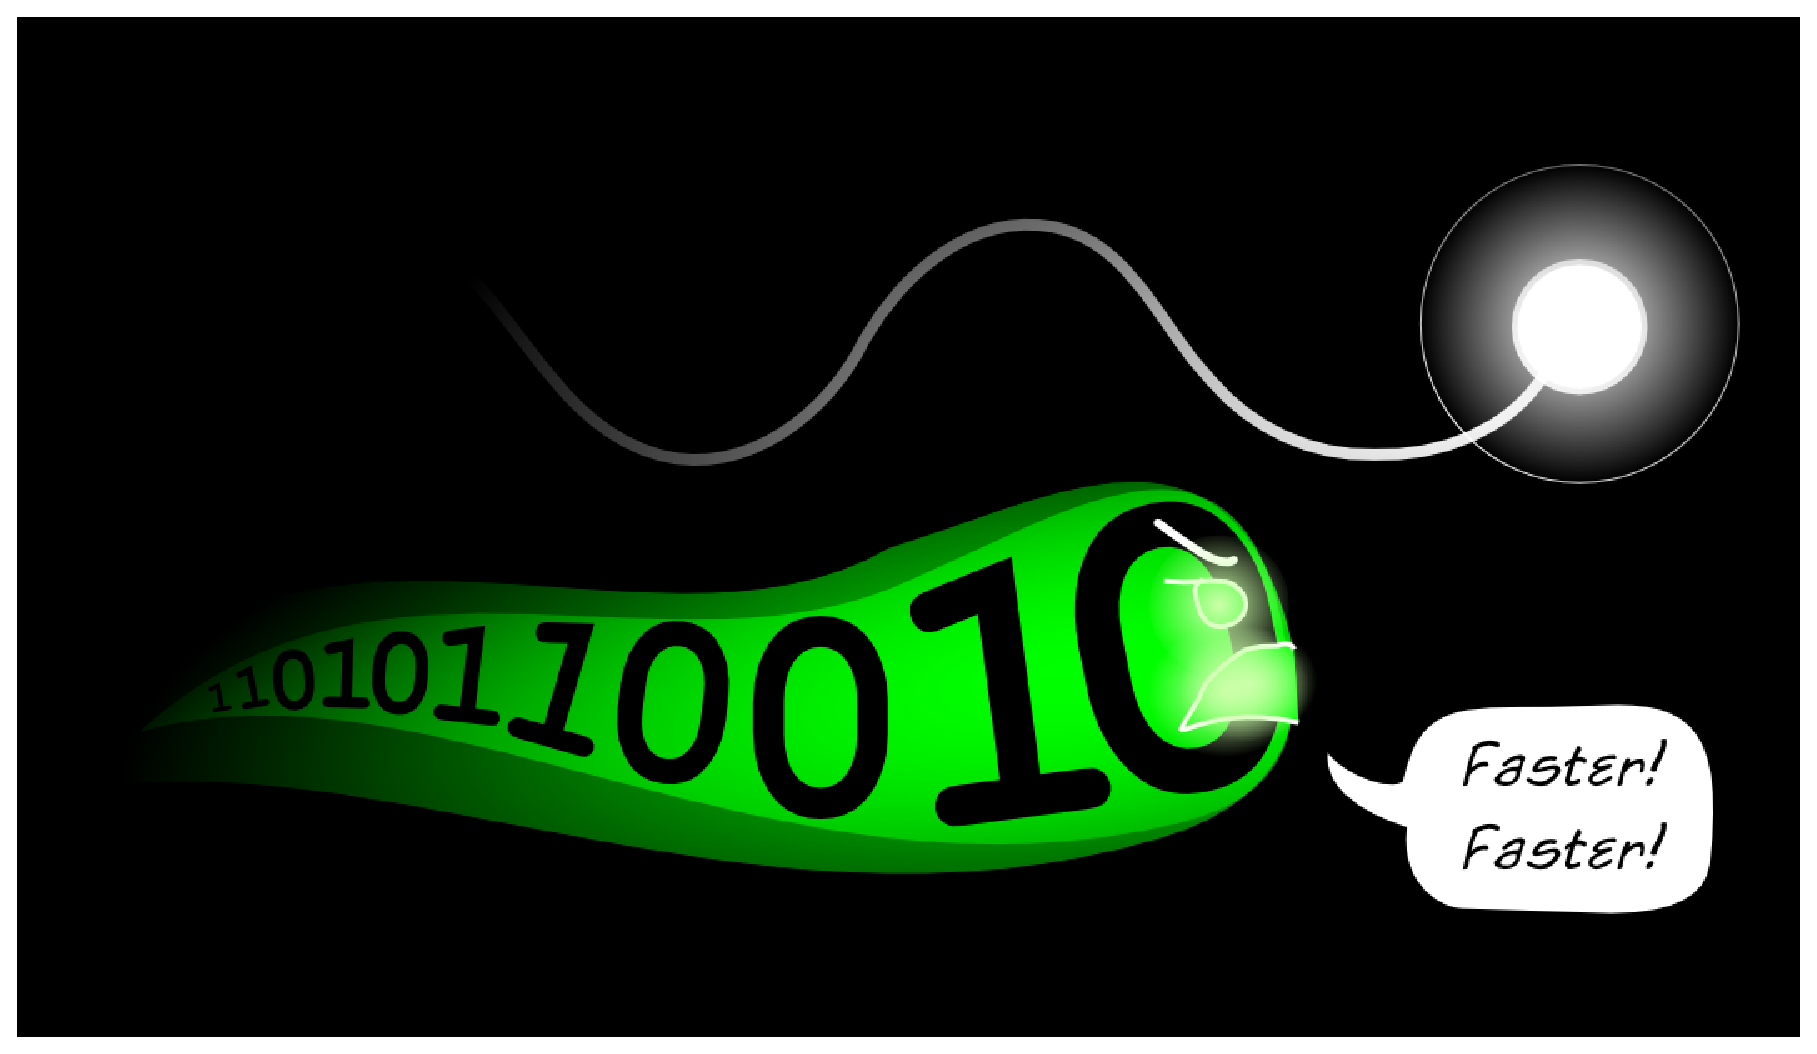
\includegraphics{cartoons/Data-chasing-light-wave}}
\caption{Hardware and Software: On Same Side}
\ContributedBy{Figure}{fig:cpu:Hardware and Software: On Same Side}{Melissa Broussard}
\end{figure}

짧게 말해서, 하드웨어와 소프트웨어 엔지니어들은 사실
Figure~\ref{fig:cpu:Hardware and Software: On Same Side} 에 우리의 데이터
스트림이 빛의 속도를 넘으려 노력하는 그림으로 나타내는 것처럼, 같은 편에서
컴퓨터들이 물리적 법칙에도 불구하고 더 빨리 동작할 수 있도록 고군분투하고
있습니다.
다음 섹션은 하드웨어 엔지니어들이 할수도 (또는 안할수도) 있는, 가능한 것들에
대해 알아봅시다.
이 싸움에서 소프트웨어가 할 수 있는 공헌은 이 책의 남은 챕터들에서 이야기
합니다.

\iffalse
In short, hardware and software engineers are really fighting on the same
side, trying to make computers go fast despite the best efforts of the
laws of physics, as fancifully depicted in
Figure~\ref{fig:cpu:Hardware and Software: On Same Side}
where our data stream is trying its best to exceed the speed of light.
The next section discusses some additional things that the hardware engineers
might (or might not) be able to do, depending on how well recent
research translates to practice.
Software's contribution to this fight is outlined in the remaining chapters
of this book.
\fi
